\begin{frame}
    \frametitle{Arbeitsablauf}
    \begin{columns}
        \begin{column}{0.50\textwidth}
            \centering
            \tikzstyle{block} = [ draw,fill=blue!20,text width=3em,align=center,
                                  minimum height=4em]
            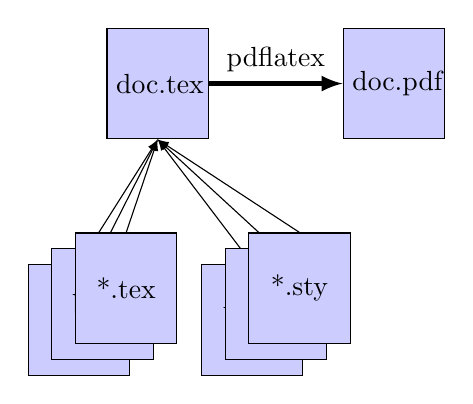
\begin{tikzpicture}
                \uncover<1->{\node[block] at (1.0,3.0) (doc-tex) {doc.tex};}
                \uncover<1->{\node[block] at (0.0,0.0) (c-tex)   {c.tex};}
                \uncover<1->{\draw[-latex] (c-tex.north)   -- (doc-tex.south);}
                \uncover<1->{\node[block] at (0.3,0.2) (b-tex)   {b.tex};}
                \uncover<1->{\draw[-latex] (b-tex.north)   -- (doc-tex.south);}
                \uncover<1->{\node[block] at (0.6,0.4) (a-tex)   {*.tex};}
                \uncover<1->{\draw[-latex] (a-tex.north)   -- (doc-tex.south);}
                \uncover<2->{\node[block] at (2.2,0.0) (b-sty)   {b.sty};}
                \uncover<2->{\draw[-latex] (b-sty.north) -- (doc-tex.south);}
                \uncover<2->{\node[block] at (2.5,0.2) (a-sty)   {a.sty};}
                \uncover<2->{\draw[-latex] (a-sty.north)   -- (doc-tex.south);}
                \uncover<2->{\node[block] at (2.8,0.4) (lay-sty) {*.sty};}
                \uncover<2->{\draw[-latex] (lay-sty.north)   -- (doc-tex.south);}
                \uncover<4->{\node[block] at (4.0,3.0) (doc-pdf) {doc.pdf};}
                \uncover<3->{\draw[-latex,ultra thick] (doc-tex.east) -- node[above] {pdflatex} (doc-pdf.west);}
            \end{tikzpicture}
        \end{column}
        \begin{column}{0.50\textwidth}
            \begin{block}{Vom getippten Text zum Dokument}
                \begin{itemize}
                    \uncover<1->{\item *.tex}
                    \uncover<2->{\item *.sty}
                    \uncover<3->{\item pdflatex}
                    \uncover<4->{\item *.pdf}
                \end{itemize}
            \end{block}
        \end{column}
    \end{columns}
\end{frame}
